\newcommand{\highlightbox}[2]{%
    \colorbox{cyan!20}{%
        \parbox{#1}{\vspace{0.5em}\centering #2\vspace{0.5em}}%
    }%
}

\chapter{Suchproblem und Suchalgorithmen}

Ein Agent muss für ein bestimmtes Ziel die richtige Wahl an Aktionen treffen und vorausplanen. Der Prozess für die Findung der Sequenz an Aktionen wird als Suche bezeichnet und durch Suchalgorithmen gefunden. Für das Finden benötigt der Agent einen Raum mit Regeln und Informationen, der im Suchproblem definiert wird. Die Informationen des folgenden Kapitel basieren auf den wissenschaftlichen Arbeiten \autocite{RN2020}, \autocite{4082128} und \autocite{Felner2011}.


\section{Suchproblem}

Ein Suchproblem wird definiert über einen Satz an möglichen Zuständen (\textit{states}), einen Ausgangszustand (\textit{initial state}), Zielzustände (\textit{goal states}), Aktionen (\textit{actions}), Übergangsmodel (\textit{transition model}) und Aktion-Kosten (\textit{action costs}).

Die Zustände beschreiben dabei die Umwelt und einen Ausgangszustand $s$, aus welchem der Agent startet. Ein Agent bekommt ein oder mehrere Ziele die in Zielzuständen beschrieben werden.

\[
\highlightbox{0.9\textwidth}{$
    \begin{aligned}
			s = \{AtCover, GunLoaded, PlayerAlive\}
    \end{aligned}
$}
\]

Die Aktionen die ein Agent besitzt können in bestimmten Zuständen $ACTIONS(s)$ ausgeführt werden.

\[
\highlightbox{0.9\textwidth}{$
    \begin{aligned}
			ACTIONS(GunLoaded) &= \{Shoot\} \\
			ACTIONS(\lnot GunLoaded) &= \{Reload\}
    \end{aligned}
$}
\]

Ein Übergangsmodell $TRANSITION(s,a) = s^*$ beschreibt dabei den resultierenden Zustand $s^*$ der durch Aktionen $a$ im derzeitigen Zustand $s$ resultiert.

\[
\highlightbox{0.9\textwidth}{$
    \begin{aligned}
			TRANSITIONS(GunLoaded, Shoot) &= \lnot PlayerAlive
    \end{aligned}
$}
\]

Durch eine Aktion-Kosten Funktion $ACTIONCOST(s,a,s^*)$ erhalten wir die Kosten einer Aktion $a$, welche in einem Zustand $s$ ausgeführt werden und in einen neuen Zustand $s^*$ resultieren.

Die Lösung für ein Suchproblem ist dabei ist die Sequenz an Aktionen, also der Plan der vom Ausgangszustand zum Zielzustand führen soll. Der gewählte Pfad sollte die geringsten Kosten von allen möglichen Lösungen haben und somit eine optimale Lösung darstellen. Der Satz an möglichen Zuständen kann dabei als Graph dargestellt werden, wobei die Kanten als Aktionen und die Knoten als Zustände dargestellt werden.


\section{Suchalgorithmen}

Das Suchproblem soll mit seinen Informationen durch einen Suchalgorithmus gelöst werden. Ein Suchalgorithmus erzeugt aus dem Suchproblem einen Suchbaum. Wie beim Graphen besteht ein Suchbaum aus Knoten $n$ und Kanten $a$, welche zu weiteren Knoten führen. 


\subsection{Knoten eines Suchbaums}

Ein Knoten speichert dabei:
\begin{itemize}
	\item Einen Zustand, zu dem die Aktion des jeweiligen Knoten geführt hat
	\item Eine Aktion, die auf dem Eltern-Knoten ausgeführt wurde
	\item Einen Eltern-Knoten, auf dem die Aktion durchgeführt wurde und den jeweiligen Knoten generiert hat
	\item Die Pfad-Kosten, der die summierten Kosten vom Ausgangsknoten bis zum jeweiligen Knoten speichert
\end{itemize}
Der Wurzelknoten ist dabei der Ausgangszustand des Agenten. Der Suchbaum beschreibt dabei Pfade zu Knoten und Ziel-Knoten, wobei mehrere Pfade zum selben Zustand führen können, jedoch jeder Knoten im Suchbaum einen eindeutigen Pfad zurück zur Wurzel hat.


\subsection{Expansion eines Suchalgorithmus}

Bei der Expandierung schaut sich der Suchalgorithmus über die $TRANSITIONS(n)$ -Funktion alle möglichen Kanten $ACTIONS(n)$ für den derzeitigen Knoten $n$ an.Zu den Kanten werden die dazugehörigen Kind-Knoten generiert, welche in eine offene-Liste hinzugefügt werden. Der Suchalgorithmus bestimmt den nächsten zu expandierenden Knoten aus der offenen Liste basierend auf dem jeweiligen Suchverfahren und dessen Bewertungsfunktion $f(n)$.

Im Bereich der Suchalgorithmen wird zwischen informierten und uniformierten Algorithmen unterschieden. Informierte Algorithmen können dabei die Distanz zum Ziel über eine Heuristik schätzen, während uniformierte eine solche Schätzung nicht durchführen können. Unter die uninformierten Suchalgorithmen fallen beispielsweise die Breitensuche, Dijkstra und Tiefensuche. Zu den informierten Suchalgorithmen gehören unter anderem \textit{Greedy best-first-search} und der A* Algorithmus. Informierte Suchalgorithmen können einen Pfad durch die Informationen der Heuristik effizienter finden, als uninformierte Suchalgorithmen.

\begin{figure}[h]
  \centering
  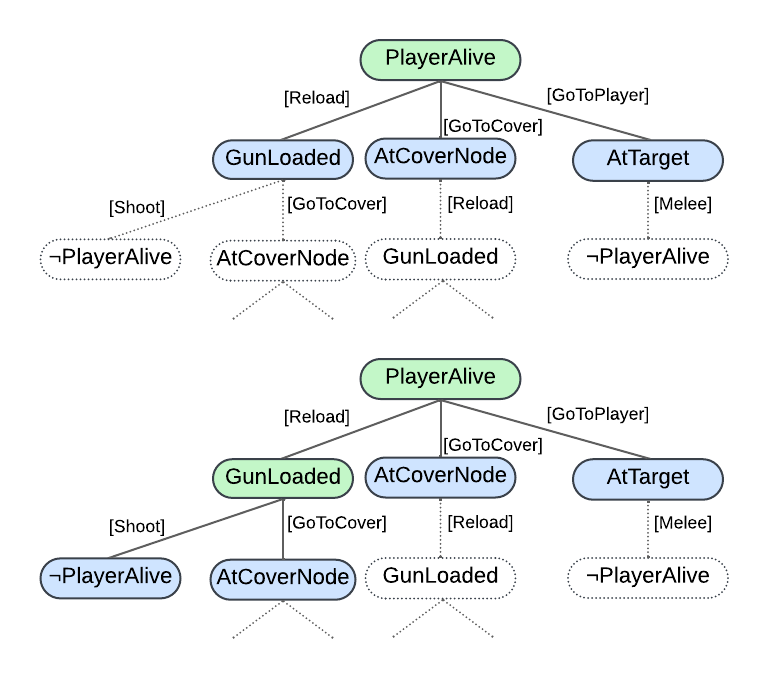
\includegraphics[width=15cm]{Suchalgorithmen/SAS}
	\captionsetup{justification=justified, format=plain}
  \caption{Suchbaum: Fängt vom Ausgangszustand an und soll den Zielzustand $\lnot \textit{PlayerAlive}$ erreichen. Grüne Knoten sind expandierte Knoten, welche in eine geschlossene Liste hinzugefügt werden. Blaue Knoten sind offene gefundene Nachbarknoten aus der offenen-Liste. Gestrichelte Knoten sind nicht entdeckte Knoten. Im Falle des Beispiels hat sich der Suchalgorithmus für den Knoten GunLoaded entschieden, da dieser optimaler als andere Nachbarknoten ist. Von dort aus ist der Zielzustand erreichbar und der Algorithmus würde eine Sequenz von Aktionen geben: \textit{[Reload,Shoot]}}
  \label{Suchalgorithmen}
\end{figure}
\clearpage

\subsection{A* Algorithmus}

Gehört zu den informierten und heuristischen Suchverfahren. Er ist ein so genannter vollständiger Algorithmus und findet einen Pfad zur Lösung, wenn einer vorhanden ist. Der Einsatz des Algorithmus wird oft für Routenplaner benutzt. So benutzt Godot 4.3 den A* Algorithmus für die Navigation. Der GOAP benutzt A* für das Suchen einer optimalen Sequenz an Aktionen.

\subsubsection{Bewertungsfunktion}

Suchalgorithmen, wie A* benutzen eine Bewertungsfunktion $f(n)$, welche dazu dient die Priorität eines Knoten $n$ während der Suche zu bewerten. Es werden dabei alle Pfad-Kosten $g(n)$ vom Ausgangsknoten bis zu Knoten $n$ mit der Heuristik $h(n)$ des Knoten $n$ bis zum Zielknoten summiert.

\[
\highlightbox{0.9\textwidth}{$
    \begin{aligned}
			f(n) = g(n) + h(n)
    \end{aligned}
$}
\]

Mit jeder Erweiterung des Pfades $n$ zu $n^{\ast}$ steigen die Kosten $g(n)$, was an den positiven tatsächlichen Aktion-Kosten $ACTIONCOST(n,a,n^*)$ der Knoten liegt.

\[
\highlightbox{0.9\textwidth}{$
    \begin{aligned}
			g(n) + ACTIONCOST(n,a,n^*) + h(n^*) &= g(n^*) + h(n^*)
    \end{aligned}
$}
\]

\subsubsection{Heuristik}

Ein Suchalgorithmus sollte einen Pfad mit möglichst geringen Kosten (\textit optimalen-Pfad) zum Ziel finden. Ob A* einen optimalen Pfad findet richtet sich nach den Eigenschaften der Heuristik $h(n)$. Eine Heuristik hat die Eigenschaften der Zulässigkeit und Konsistenz.
Bei einer zulässigen Heuristik werden die Kosten stets unterschätzt oder genau geschätzt. Sie bleibt im Intervall $[0, h^{\ast}(n)]$ wobei $h^{\ast}(n)$ die tatsächlichen Kosten sind.

\[
\highlightbox{0.9\textwidth}{$
    \begin{aligned}
			0 \leq h(n) \leq h^*(n)
    \end{aligned}
$}
\]

Eine konsistente Heuristik, muss gleichzeitig zulässig sein und die Dreiecksungleichung erfüllen. Umgekehrt muss eine zulässige Heuristik nicht konsistent sein. So muss diese die Dreiecksungleichung erfüllen, welche besagt, dass die Heuristik $h(n)$ geringer sein soll als die Summe der Aktion $a$ und die Heuristik des folgenden Knoten $h(n^*)$.

\[
\highlightbox{0.9\textwidth}{$
    \begin{aligned}
			h(n) \leq ACTIONCOST(n,a,n^*) + h(n^*)
    \end{aligned}
$}
\]

Die konsistente Heuristik hat eine stärkere Eigenschaft als eine zulässige Heuristik. Der expandierte Knoten bei einer konsistenten Heuristik wird optimal sein, wodurch wir diesen Knoten nicht erneut in die offene-Liste hinzufügen müssen.

Mit einer inkonsistenten Heuristik können Pfade auftreten, welche denselben Zustand erreichen. Somit können mehrere Pfade mit unterschiedlichen Kosten aber selben Zustand in der offenen Liste auftreten, was zur höheren Zeit und Speicherkosten führt.

\subsubsection{Beweis für Optimalität}

Arbeitet der A* Algorithmus mit einer zulässigen oder konsistenten Heuristik, so wird diese den optimalen, kostengünstigsten Pfad zu einem Ziel finden.

Vorraussetzung:
\begin{itemize}
\item A* expandiert auf Knoten mit der geringsten $f(n)$
\item Wir haben zwei mögliche Zielknoten:
\begin{itemize}
	\item optimaler Zielknoten: $G_o$
	\item suboptimaler Zielknoten: $G_s_o$
\end{itemize}
\item Eine zulässige Heuristik: $0 \leq h(n) \leq h^*(n)$
\item Einen nicht expandierten Knoten: $n$
\end{itemize}

Beweis:
\begin{enumerate}
	\item Da keine weiteren Schritte vom Zielzustand möglich sind gilt: $h(G_o) \land h(G_s_o) = 0$
	\[
	\highlightbox{0.9\textwidth}{$
		\begin{align*}
			f(G_o) &= g(G_o) + h(G_o) \\
			f(G_o) &= g(G_o) \\
			f(G_s_o) &= g(G_s_o) + h(G_s_o) \\
			f(G_s_o) &= g(G_s_o)
		\end{align*}
	$}
	\]
	
	Da $G_s_$ suboptimal ist folgt, dass die Pfadkosten $f(n)$ von $G_s_o > G_o$ sind und somit: $f(G_s_o) > f(G_o)$.
	\item Da $g(G_o)$ der tatsächliche Zielknoten ist und $h^*(n)$ die tatsächlichen Kosten von $G_o$ sind gilt:
	\[
	\highlightbox{0.9\textwidth}{$
    \begin{align*}
			f(n) = g(n) + h(n) &< g(n) + h^*(n) = g(G_o) \\
			f(n) &< g(G_o)
		\end{align*}
	$}
	\]
\end{enumerate}
Aus 1. und 2. folgt: $f(n) < f(G_o) < f(G_s_o)$. Somit würde A* nicht zu $G_s_o$ führen und ist mit einer zulässigen Heuristik optimal.

\begin{figure}[h]
  \centering
  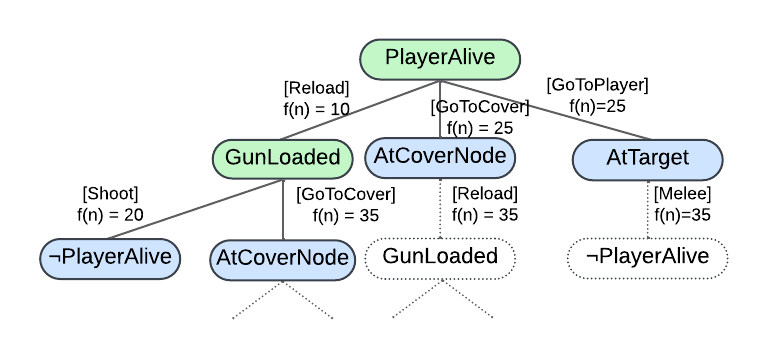
\includegraphics[width=15cm]{Suchalgorithmen/A_Erweiterung}
	\captionsetup{justification=justified, format=plain}
  \caption{A Suchalgorithmus: Der Pfad \textit{[Reload,Shoot]} hat mit $f(n)=20$ die geringsten Pfadkosten. Das Beispiel kommt aus  Abbildung 1.1. Wie genau $g(n)$ und $h(n)$ am Beispiel von NPC-Aktionen berechnet wird, wird im GOAP Kapitel erklärt.}
  \label{Suchalgorithmen}
\end{figure}